\documentclass[a4paper,11pt]{kth-mag}
\usepackage[T1]{fontenc}
\usepackage{textcomp}
\usepackage{lmodern}
\usepackage{graphicx}
\usepackage[utf8]{inputenc}
\usepackage[swedish,english]{babel}
\usepackage{modifications}
\usepackage{algorithmicx}
\usepackage{algpseudocode}

% http://library.uwl.ac.uk/find/guides/general/harvard_reference.html

\title{Comparison of Artificial Brains in Simulating Animal Behaviour}
\subtitle{Comparing radial basis, linear and random functions for decision-making}
\foreigntitle{Titel pa svenska}
\author{Björn Tegelund\\Johan Wikström}
\date{November 2003}
\blurb{Bachelor's Thesis at CSC\\Supervisor: Petter Ögren\\Examiner: Mårten Björkman}
\trita{TRITA xxx yyyy-nn}
\begin{document}
\frontmatter
\pagestyle{empty}
\removepagenumbers
\maketitle
\selectlanguage{english}
\begin{abstract}
  This is a skeleton for KTH theses. More documentation
  regarding the KTH thesis class file can be found in
  the package documentation.

\end{abstract}
\clearpage
\begin{foreignabstract}{swedish}
  Denna fil gfwfqwfwqfqer ett avhandlingsskelett.
  Mer information om \LaTeX-mallen finns i
  dokumentationen till paketet.

\end{foreignabstract}
\clearpage
\tableofcontents*
\mainmatter
\pagestyle{newchap}
\chapter{Introduction}

\section{Background}

Genetic algorithms are algorithms that emulate evolution to achieve a optimal solution to a problem\footnote[1]{Proof}. 
These algorithms have many uses and we wanted to investigate whether the phenomena which occur in nature
due to evolution also occurs when using genetic algorithms. In nature evolution has spawned a wide variety
of survival strategies such as adaptation, camouflage colours and mimicry. Genetic algorithms however, are 
very simplified mathematical models of these mechanisms which means that these phenomena might not occur 
at all.

\section{Scope and Objectives}

Our main objective is to compare brains for simulating animal behaviour using radial-basis functions and linear functions. As a baseline we will also use brains which make random decisions. To train our animals we use genetic algorithms. The genetic algorithms provide the genes which will then be used in their brains to make decisions. We will look at statistics such as learning speed, execution speed and how well they can adapt to their surroundings.

The animals will be given different tasks to do in each experiment, ranging from simply gathering food to avoiding predators to mimicking things in the world to survive. In each experiment the three brain architectures are compared and contrasted. By doing these simulations we wish to find the pros and cons for both brains using radial-basis functions and linear functions, when used for artificial intelligence in this way. We also wish to find how complex of a task a brain using linear functions is able to solve, and in the cases where it is not able to solve the problem completely we wish to know how much better is it than the random brain.

% TODO: What did we manage to simulate?
%  Forcing them to adapt certain genetic phenomena such as adaptation (learning), co-evolution and extinction, mimicry, group forming and co-operation prioritised in the order presented (as increasingly complex behaviour and difficulty to simulate).

\section{Achievements}

\chapter{Technical Overview}

\section{Genetic Algorithms}

\subsection{Overview}
What are genetic algorithms?\\
How are they typically used?\\
How do they relate to genetics and evolution?\\
Overview of algorithm\\

Genetic algorithms are a way of approximating solutions to NP-hard problems, a group of problems that are extremely computationally expensive. They are a form of machine learning algorithms typically used to solve problems with a large or complex search space and where other machine learning algorithms fail \cite{marsland}. Genetic algorithms mimic natural selection in nature by defining a set of genomes, or individuals, where each genome represents a possible solution to the given problem. This genome is commonly stored as a string of 0:s and 1:s or as a list of floating point values. This set of genomes undergoes several iterations, or generations, of small improvements by fitness evaluation, selection , mutation and crossover. These operators all have equivalents in real evolution and eventually, the genomes will converge to a solution which represents a local minima in the search space. The advantage of genetic algorithms is that the crossover operator enables a wider search over the problem domain than many other approaches, using less calculations \cite{holland}. In the following subsections, the most crucial parts of the genetic algorithm will be explained and in figure \ref{algorithm-overview} we depict an overview of the genetic algorithm in pseudo code.

\begin{figure}
\begin{algorithmic}
\State $ S \gets $ a random distribution of genes
    \While {the genes have not converged towards a solution}

        \State $F\gets fitness(S)$
		\Comment Calculate fitness values for all $s \in S$
		\State $X \gets select(S,F)$
		\Comment Get a multiset of S using fitness values
		\State $C \gets crossover(X)$
		\Comment Apply crossover operator on multiset
		\State $M \gets mutate(C)$
		\Comment Apply mutation operator on crossed genes
		\State $S \gets M$
		\Comment Restart with the new generation
    \EndWhile
\end{algorithmic}
\caption{An overview of the genetic algorithm used in the experiments}
\label{algorithm-overview}
\end{figure}

\subsection{Fitness}
Fitness is the only means of measuring the success of the solution. In nature, fitness is simply determined by the number of offspring produced by the individual and the percentage of that offspring which survives long enough to generate new offspring. In genetic algorithms however, the fitness function can be any value that describes each individual's success at solving the problem at hand \cite{marsland} and genetic algorithms can get significant performance advantages by simply selecting the correct fitness function. The fitness function should be strictly positive for all inputs and preserve some form of relative internal ordering of the individuals. In most problems there are multiple choices of fitness functions and the best choice of fitness function is unique for every problem. For this reason, we experimented with different fitness functions before settling for simply the life length of our individuals.
\subsection{Selection}
Selection is the process of selecting which organsims that should be allowed to reproduce and in what proportions. In nature, selection is closely tied to fitness, the fittest individual is also "selected" most often, but in genetic algorithms there are several different ways to model this selection process. A good fitness function should strike a balance between favorizing the fittest individuals and allowing less fit individuals to survive in a reduced number.  One trivial selection function could be to simply select all individuals that pass a certain fitness threshold \cite{marsland} [TROR DET STOD DÄR IAF]. This is a bad idea, however, since there are few ways to determine the correct threshold value. In the beginning of the evolution, a high threshold will exclude most of the genes due to low general fitness and this will lead to a fast reduction of genetic variation. In the later stages of the evolution all individuals will pass the threshold, rendering the selection function useless.

A better approach is the so called roulette wheel selection where each individual is mapped to an area of a "roulette wheel". A larger fitness value means a larger area on the roulette wheel and the selection function simply generates random values corresponding to the areas of this roulette wheel. In this way, the individuals are chosen based on a biased stochastic variable and there is room for individuals with high fitness to dominate as well as for individuals with low fitness to be included by chance.

Undrar om vi ska skriva något om NSGA II...
 
\subsection{Mutation}
Mutation is a random, usually small, change of an individuals genome. In nature In genetic algorithms it is usually implemented as a small probability for each gene to mutate. When the genome consists of a series of 0:s and 1:s, the mutation operator is simply a flip of that bit and when the genes consist of floating point values, the mutation can be an addition or multiplication of a random value. If the mutation rate is too high, it becomes very hard to reach convergence since the good solutions are mutated into averaged solutions.

\begin{figure}
\centering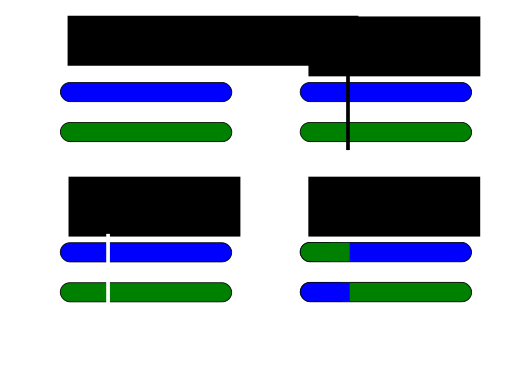
\includegraphics[scale=0.5]{crossover}
\caption{A schematic drawing showing crossover of two genomes.}
\label{crossover-figure}
\end{figure}

\subsection{Crossover}
Crossover is the operation of combining two genomes into two new genomes. One common crossover operator is known as  single point crossover and it consists of splitting two genomes at the same position and merging the splitted parts into two new genomes. The split position is chosen randomly and the two new genomes share no genes with each other. This process is displayed in Figure \ref{crossover-figure} There is also multiple point crossover where there are multiple splitting positions as well as uniform crossover where each gene can be exchanged with a certain probability.




\section{Radial Basis Functions}
\subsection{Overview}

\begin{figure}
%\centering\includegraphics[scale=0.5]{rbf_1d.png}
\caption{Three one-dimensional RBFs with varying $\mu$ and $\sigma$ values.}
\end{figure}

A radial basis function (RBF) is a bell-shaped function whose value depends on the distance from some origin, denoted $\mu$ in the formula.  Radial basis functions are commonly used in neural networks as a way to encode input information. They are favourable to use as they have locality, something which linear functions do not. In particular they are used for function approximation, as any function can be approximated as the sum of a number of weighted radial basis functions. A property of radial basis functions which can both be interpreted as an advantage and disadvantage is that their value never exceeds a given constant, compared to a linear function which can grow to infinitely high or low numbers.

Radial basis functions are commonly implemented using a formula such as \ref{RBF_1}, which is a three-dimensional function centred around $(\mu _{x}$, $\mu _{y}$, $\mu _{z})$. The width of the bell-curve in each dimension is determined by $\sigma _{x}$, $\sigma _{y}$ and $\sigma _{z}$ respectively.

\begin{figure}
\begin{equation}
f(x,y,z) = \exp(-(\frac{(x-\mu_{x})^{2}}{2 \sigma _{x}^{2}})) + \exp(-(\frac{(y-\mu_{y})^{2}}{2 \sigma _{y}^{2}})) + \exp(-(\frac{(z-\mu_{z})^{2}}{2 \sigma _{z}^{2}}))
\end{equation}
\caption{A sum of three radial basis functions, corresponding to three input values.\label{RBF_1}}
\end{figure}

\chapter{Implementation}
\section{Model}
\subsection{Simulation in Python}
Square world with walls, circular inhabitants with antennae\\
Good and bad food sources\\
Predators?\\
Possible modifications to enforce different behaviour?\\
What libraries will we use? Why?\\
Optimisations?\\

\subsection{Methods of Enforcing Behaviour}
Adding input\\
Additional terms in brain calculations\\
Adding predators\\
More kinds of food\\
Being able to see more things in the world\\
Placing objects into the world\\
\subsection{Linear Decision Making}
\subsection{RBF-Based Decision Making}

When input is received by a creature, it is in form of eight numbers, four for each antenna. Three of the inputs for each antenna are the red-, green- and blue components of the currently detected object's colour. The fourth input is zero when no object is detected and one when an object is. The three colour-based inputs are then used in several three-dimensional radial basis functions. For each antenna a $\Delta r$ (change in rotation) and $\Delta s$ (change in speed) is computed by summing the function values and normalising them. The $\Delta r$ and $\Delta s$ for each antenna are then grouped and used by the creature to change it's rotation and speed. See equation \ref{RBF_decide}.

\begin{figure}
\begin{equation}
\Delta s _{left} = f(\mathbf{x} _{left})
\end{equation}
\caption{Calculating the $\Delta s$ for the left eye, using the input vector $\mathbf{x} _{left}$ corresponding to the colours of the object detected using the left antenna.\label{RBF_decide}}
\end{figure}

Each radial basis function also has a $\sigma$ and $\mu$ which are decided by the creature's genes. $\sigma$ and $\mu$ are in the ranges of $[0,1]$ and $[-1,1]$ respectively. In practice this means that the creatures' change in speed and rotation, when detecting an object in each antenna, depend on their genetic makeup.

The difference between using radial basis functions and linear functions is that you have a much larger possibility to approximate any decision-making strategy. For example an RBF-based brain could make the distinction between different shades of green and thus react differently to them, while a linear function could only decide if more green is better or worse.
\subsection{Random Decision Making}
\subsection{Genetic Algorithm}
What kind of genetic algorithm do we plan to use?\\
Fitness, crossover, mutation, selection, which ones?\\
Flow chart of our algorithm\\
NSGA-II\\
Roulette selection\\

\subsection{Experiments}
(In every experiment linear and RBF are compared, eventually mixed)\\
Interested in:\\
Time to maximal fitness\\
Highest possible fitness\\
\begin{itemize}
\item Adaptation 1. Finding and eating food
\item Adaptation 2. Finding and eating food, avoiding "bad" food
\item Co-evolution and extinction 1. Predator vs prey, prey eats food as in first experiment. (bushes are bad for predators)
\item Speciation and co-operation 1. Allow the creatures to evolve which "colour" food they can eat, attempt to create two separate species from one, one species eating green bushes and one red.
\item Mimicry 1. Making the prey mimic bushes or predators to avoid being eaten.
\item Mimicry 2. Predators attempt to mimic bushes to make prey run into them.
\item Group forming 1. Rerun all previous experiments, but with the ability to detect the nearest creature of the same species.
\end{itemize}


\chapter{Results}
\section{Simulation results}
\subsection{Observed Behaviours}
\section{Discussion}
\subsection{Constraints and problems}
Performance problems\\
Other unexpected problems?\\

\section{Conclusions and Future Work}

\begin{thebibliography}{9}
\bibitem{montana89} 
Montana, D. J.,  and Davis, L. (1989, August). Training feedforward neural networks using genetic algorithms. In \emph{Proceedings of the eleventh international joint conference on artificial Intelligence} (Vol. 1, pp. 762-767).
\bibitem{langton97}
Langton, C. G., and Shimohara, T. (Eds.). (1997). \emph{Artificial Life V: Proceedings of the Fifth International Workshop on the Synthesis and Simulation of Living Systems} (Vol. 5). Mit Press.
\bibitem{marsland}
Marsland, S. (2009). \emph{Machine Learning, an Algorithmic Perspective}. CSC-Press
\bibitem{holland}
Holland, J. H. (1992). Genetic algorithms. \emph{Scientific american, 267(1)}, 66-72.


\end{thebibliography}

\appendix
\addappheadtotoc
\chapter{RDF}\label{appA}

\begin{figure}[ht]
\begin{center}
And here is a figure
\caption{\small{Several statements describing the same resource.}}\label{RDF_4}
\end{center}
\end{figure}

that we refer to here: \ref{RDF_4}
\end{document}
